% Following colors are predefined: red, green, blue, cyan, magenta, yellow, black, gray, darkgray, lightgray, brown, lime, olive, orange, pink, purple, teal, violet and white.

\documentclass[tikz,border=1pt]{standalone}
\usetikzlibrary{shapes.misc, positioning}
\usetikzlibrary{external} 
\tikzsetexternalprefix{ffigurau} 
\tikzexternalize

\begin{document}
	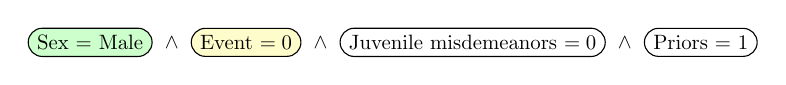
\begin{tikzpicture}[scale=1, every node/.style={scale=0.75}]
	\node (1) [fill=green!20,draw, rounded rectangle] {Sex $=$ Male};
	\node (2) [right=of 1, xshift=-12.5mm] {$\wedge$};
	\node (3) [fill=yellow!20, draw, right=of 2, xshift=-12.5mm, rounded rectangle] {Event $=0$};
	\node (4) [right=of 3, xshift=-12.5mm] {$\wedge$};
	\node (5) [fill=white, draw, right=of 4, xshift=-12.5mm, rounded rectangle] {Juvenile misdemeanors $=0$};
	\node (6) [right=of 5, xshift=-12.5mm] {$\wedge$};
	\node (7) [fill=white, draw, right=of 6, xshift=-12.5mm, rounded rectangle] {Priors $=$ 1};
	\end{tikzpicture}
\end{document}